
\chapter{Improved PyrLK Optical Flow Method}
\label{cha:pyrlk}
%----------------------------------PyrLK--------------------------------------
The first step of image-based tree modeling is 3D reconstruction, and the first
step of 3D reconstruction is character matching, which is to find a same space 
point projecting onto 2 frames. This article chooses Harris corners as the character
points, which can be affine invariant. The traditional PyrLK optical flow is rather 
limited, because:\\

\begin{itemize}
	\item \textbf{No Rotation Support} The traditional PyrLK optical flow method doesn't support
		rotation of character points, which will certainly limit its extension.
	\item \textbf{Lack Validation Methods} The traditional PyrLK lacks validation methods, which will
		lead to too many match errors, and will no doubt cause more trouble to the subsequent 3D 
		reconstruction steps.
\end{itemize}

In order to solve these two problems, this article proposes an affine transformation and back track based
PyrLK optical flow method, which can give a solution to the problems above, and ensure the robustness and 
correctness of the 3D reconstruction.

%\subsection{对于SIFT特征点匹配的尝试}
%对于特征点的匹配,本文首先尝试的是利用VisualSFM工具自带的SIFT特征点匹配。
%但是经过大量实验发现,该工具自带的SIFT特征点匹配并不能很完整地找到匹配的
%点对,从而导致了三维重建所依赖的数据不足、不精确,最后重建出来一个缺失度
%很大的模型,这样的模型显然不能成功的进行骨架抽取。
%
%根据实验结果分析,除开

\section{Optical Flow Introduction}
The concept of optical flow is proposed by James Gibson. 1981, Horn and Schunck connect the 
2D velocity field with the gray scale creatively and provided an effective calculation method
for optical flow\cite{horn}. They assume the light intensity stay invariant, and the grayscale
of the image changes as the background or target moves. Under such assumption, the optical flow
method detects the target motion through different velocity of target and background.

Moreover, when the objects in 3D scene move against the 2D image plane, the projection on 2D image
plane forms the motion, which turns out to be optical flow when it is represented in the grayscale mode.
In other words, the optical flow is the immediate velocity of the object on the view plane, which is 
measured by the displacement of pixels in the image. The optical flow filed is the set of optical flow
point and is a 2D immediate velocity field. It can represent the displacement of the whole image, which
can be used to detect the motion of 3D targets.

After optical flow method was proposed, many scholars have studied on it and improved it. Each method has
its advantages, and the efficiency and applications vary. One of the most typical one is the Lucas-Kanade
local smooth method(LK optical flow)\cite{lk}, which uses differential of time and space to calculate the 
speed vector and smooth out the image to track the optical flow. And in 2000, Jean-Yves proposed a pyramidial
implementation of LK optical flow method, which is called PyrLK optical flow method\cite{pyrlk}.

\section{PyrLK Optical Flow method}
\label{subsec:pyrlk}
Assume the value function of pixels is $I(x,y,t)$,which indicates the value of pixel on $(x,y)$ is $I(x,y,t)$
at time $t$. So after $\Delta t$,the pixel value will change to $I(x+\Delta x,y+\Delta y, t+\Delta t)$。
Here is the reduction:\\
\[  I(x+\Delta x,y+\Delta y, t+\Delta t)=I(x,y,t) + \frac{\partial I}{\partial x}\Delta x 
		+ \frac{\partial I}{\partial y}\Delta y + \frac{\partial I}{\partial t}\Delta t \]
\begin{displaymath}
	\begin{array}{cc}
		\implies & \frac{\partial I}{\partial x}\Delta x 
		+ \frac{\partial I}{\partial y}\Delta y + \frac{\partial I}{\partial t}\Delta t = 0\\
		\implies & \frac{\partial I}{\partial x}V_x 
		+ \frac{\partial I}{\partial y}V_y + \frac{\partial I}{\partial t} = 0 
	\end{array}
\end{displaymath}
\begin{equation}\label{eq:opticalflow}
	\begin{array}{cc}
				\implies & I_xV_x + I_yV_y = -I_t
	\end{array}
\end{equation}

Lucas-Kanade Optical Flow is based on principles above, and it assumes that the displacement between
two frames is small, and it stays constant in a neighborhood region. Under such assumptions, an equation
set can be listed: \\
\begin{equation}
	\left\{
		\begin{array}{c}
			I_x(q_1)V_x + I_y(q_1)V_y = -I_t(q_1)\\
			I_x(q_2)V_x + I_y(q_2)V_y = -I_t(q_2)\\
			\vdots\\
			I_x(q_n)V_x + I_y(q_n)V_y = -I_t(q_n)\\
		\end{array}
	\right.
\end{equation}

The $q_1,q_2,...,q_n$ is the points in local window,And $I_x(q_i),I_y(q_i),I_z(q_i)$ is the partial derivative
at $q_i$ of image $I$ in direction $x,y,t$, which can be written in matrix form:
\begin{equation}
	A=	
	\left(
	\begin{array}{cc}
		I_x(q_1) & I_y(q_1)\\
		I_x(q_2) & I_y(q_2)\\
		  \vdots & \vdots\\
		I_x(q_n) & I_y(q_n)
		\end{array}
	\right),\quad
	v=
	\left(
	\begin{array}{c}
		V_x\\
		V_y
	\end{array}
	\right),\quad
	b=
	\left(
	\begin{array}{c}
		-I_t(q_1)\\
		-I_t(q_2)\\
		\vdots\\
		-I_t(q_n)
	\end{array}
	\right)
\end{equation}

The number of unknowns is far greater than the number of equations, so $A$ is over determined, LK optical flow
uses the least squares method to calculate the optical flow velocity. 

Although the LK optical flow method is intuitive, there is a problem. The motion block detected is positive correlation,
so in order to catch the motion of big block, it's supposed to largen the size of window. But as the size of window increases,
the velocity should keep stable in a larger region, which is against the assumption of the method. The pyramidial implementation
of Lucas-Kanada method solves this problem, and its ideas are given below:\\

Assume $I$ and $J$ are two grayscale images,$I(x)$ and $J(x)$ is the grayscale value at $(x,y)$ in $I$ and $J$。Consider a point
$\mathbf{u}=(u_x, u_y)$ on image $I$,The goal of character tracking is to find a corresponding point $\mathbf{v}
=\mathbf{u}+\mathbf{d}=(u_x+d_x,u_y+d_y)$ on J,which makes that $I(\mathbf{u})$ and $J(\mathbf{v})$ are similar。Vector
$\mathbf{d}=(d_x,d_y)$ is the optical flow velocity at point $\mathbf{x}$。Then the similarity of the neighborhood is defined,
assume $\omega_x$ and $\omega_y$ are two integers,the velocity is the vector $\mathbf{d}$ which lets the formula reach its minimum:\\
\begin{equation}\label{eq:similarity}
	\epsilon(\mathbf{d})=\epsilon(d_x,d_y)=\sum_{x=u_x-\omega_x}^{u_x+\omega_x}\sum_{y=u_y-\omega_y}
	^{u_y+\omega_y}(I(x,y) - J(x+d_x,y+d_y))^2.
\end{equation}
The size of neighbor window is $(2\omega_x+1)\times(2\omega_y+1)$。This formula indicates to find a vector $\mathbf{d}$
letting the difference of $\mathbf{u}$ and $\mathbf{v}$ reach minimum in neighborhood region。

Then this method uses the pyramidial representation of image, which uses the source image as the highest resolution level,
and iteratively downsamples the image, one new resolution level can be got after each iteration. By doing this, the constant
window size can map to a larger area in low resolution image, and the big block motion is supported then.

\section{Improved PyrLK Optical Flow Method}
\label{subsec:revisedpyrlk}
\subsection{Support Affine Transformation}
The PyrLK optical flow method has already worked well on translation-oriented match. However, this is not the best way
to solve the matching problems on trees. Because the two adjacent frames are taken from two diffrent angles, so the character
points should have some transformation motion. However, this is not solved in traditional PyrLK method. Therefore, there is 
need to extend the method to support affine transformation.

Assume two points fit the affine matrix $A$,So:\\
\begin{equation}
	\left(
	\begin{array}{c}
		\Delta x'\\
		\Delta y'\\
		0
	\end{array}
	\right)
	=
	\left(
	\begin{array}{ccc}
		a_{11} & a_{12} & a_{13}\\
		a_{21} & a_{22} & a_{23}\\
				0 & 0 & 0
	\end{array}
	\right)
	\cdot
	\left(
	\begin{array}{c}
		\Delta x\\
		\Delta y\\
		1
	\end{array}
	\right)
\end{equation}
Take that to equation \ref{eq:opticalflow}:\\
\begin{equation}
	(a_{11}\ a_{12}\ a_{13}\ a_{21}\ a_{22}\ a_{23})\cdot
	\left(
	\begin{array}{c}
		\frac{\partial I}{\partial x}\Delta x\\
        \frac{\partial I}{\partial x}\Delta y\\
        \frac{\partial I}{\partial x}\\
        \frac{\partial I}{\partial y}\Delta x\\
        \frac{\partial I}{\partial y}\Delta y\\
        \frac{\partial I}{\partial y}\\
	\end{array}
	\right)
	=-I_t
\end{equation}

Matrix $A$ can be sovled by using the least squares method.

Modify the definition equation \ref{eq:similarity} to support the affine transformation:\\
\[ Let\quad \mathbf{a_1}=(a_{11},a_{12},a_{13})\quad \mathbf{a_2}=(a_{21},a_{22},a_{23})\quad
\mathbf{b}=(d_x,d_y,1)\]\\
\begin{equation}\label{eq:affine}
	\epsilon(\mathbf{d})=\epsilon(d_x,d_y)=\sum_{x=u_x-\omega_x}^{u_x+\omega_x}\sum_{y=u_y-\omega_y}
	^{u_y+\omega_y}(I(x,y) - J(x+\mathbf{a_1}\cdot \mathbf{b},y+\mathbf{a_2}\cdot \mathbf{b}))^2.
\end{equation}


\subsection{Back tracking and Median Filtering}
The several previous sections are discussing the extension stuff of the method. However, how can
we make sure the two matching points really match. The traditional PyrLK method hasn't solved this
problem, which makes it unreliable. The present method lacks bidirectional check, which means that
the similarity of two matching points should be bidirectional. So this article proposes the back
tracking method to validate this quality.

Moreover, any matching algorithm can't make promises that it's perfectly matching. So after finishing
the algorithm, it should drop some "edge" matches, which can make the result more robust. This article
proposes a median filtering method, which can filter out those whose similarity is below the median line:\\

\begin{itemize}
	\item \textbf{Neighborhood Similarity Median Filtering}: After the PyrLK is conducted, for each matching pair, 
		we compute their normalized correlation as their similarity。The formular is given below:\\
		\begin{equation} \label{eq:ccoeff}
			R(x,y) = \frac{\sum_{x',y'}(T'(x',y')\cdot I'(x + x', y + y'))}
			{\sqrt{\sum_{x', y'}T'(x',y')^2\cdot \sum_{x',y'}I'(x+x',y+y')^2}}
		\end{equation}
		And then compute the median value of all the similarity, for those less than this value, we drop them.
	\item \textbf{Back Tracking Error Median Filtering}: After we conduct the back tracking,each pair will get an error value,which indicates the
		space position difference between the back track point and the source point. This article will drop those less than the median error value.
\end{itemize}

The remaining points after back tracking and median filtering will be considered as the robust match result.
Algorithm \ref{alg:backtrack} gives the pseudo-code of back tracking and median filtering:\\
\begin{algorithm}[H]
	\caption{Back Tracking \& Median Filtering}
	\label{alg:backtrack}
	\begin{algorithmic}[1]
	\Require Back Tracking Error Array $\mathbb{B}[1..n]$,Neighborhood similarity array $\mathbb{S}[1..n]$
	\Require Source matching pair array $\mathbb{P}$
	\Ensure Desitination matching pair array $\mathbb{Q}$
	\State Initialize back tracking error median value $mid_{back}$,Neighborhood similarity median value $mid_{similar}$
	\State SortArray($\mathbb{B}[1..n]$)
	\State SortArray($\mathbb{S}[1..n]$)
	\State $mid=(n+1)/2$
	\State $mid_{back}=\mathbb{B}[mid],\quad mid_{similar}=\mathbb{S}[mid]$
	\For{$i=1$ to $n$}
	\If{$\mathbb{B}[i] < mid_{back} \cap \mathbb{S}[i] > mid_{similar}$}
		\State $\mathbb{Q}.AddMatch(\mathbb{P}[i])$
	\EndIf
	\EndFor
	\State \Return $\mathbb{Q}$
	\end{algorithmic}
\end{algorithm}

\section{PyrLK with Robustness Improvement and Affine Transformation Support}
The adaptability and stability are improved a lot after PyrLK supports the affine transformation
and improves the robustness, which results in:\\
\begin{itemize}
	\item \textbf{Support Rotation}: Each two frames are the projection of 3D Rotation, so the rotation
		support is important, since it happens on every pair. By doing so, the accuracy can be improved a lot.
	\item \textbf{Matching Validation}: For each matching pair, this article uses normalized correlation to 
		calculate their similarity. Only those who pass the similarity validation can be the real mathcing pairs.
	\item \textbf{Eliminate Matching Mistakes}: Matching in only one direction can be unreliable, so this article
		uses back tracking to do bidirectional validation, which can improve the robustness of the algorithm.
\end{itemize}

Figure\ref{fig:pyrlk} gives the contradiction between the improved version and the traditional version. The images here
use different color path to represent the two adjacent frames, where the green path represents the previous picture and 
the purple path represents the next picture, and the red line indicates the matching relationship. From figure\ref{fig:pyrlk}(a)
we can find, there are bunches of errors with the traditional method for its lack of validation. For example, the trees far away
from sight should be sensitive to the rotation of camera, but figure\ref{fig:pyrlk}(a) doesn't catch this. And there are lots of
points matching to the background incorrectly. In figure\ref{fig:pyrlk}(b), the optical flow is appropriate and doesn't have the 
problems just metioned. So the improved version has an appreciative effect.
\begin{figure}[H]
	\centering
	\subfloat[Traditional PyrLK]{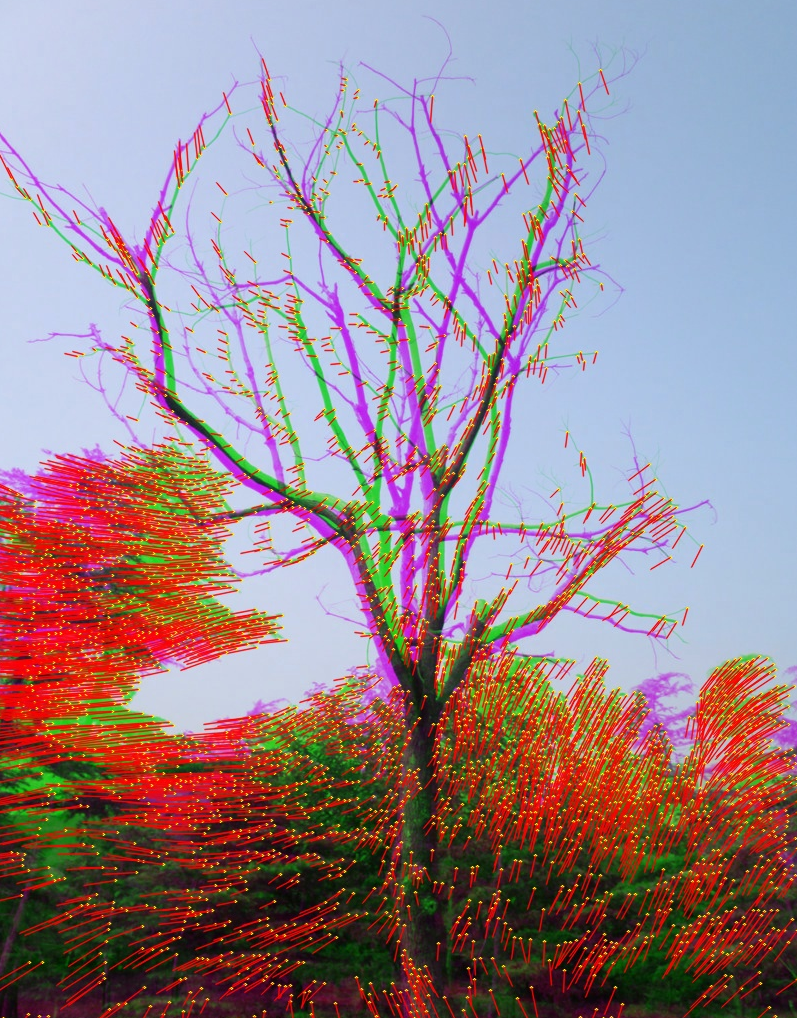
\includegraphics[height=10cm]{old.png}}\hspace{4em}
	\subfloat[Improved PyrLK]{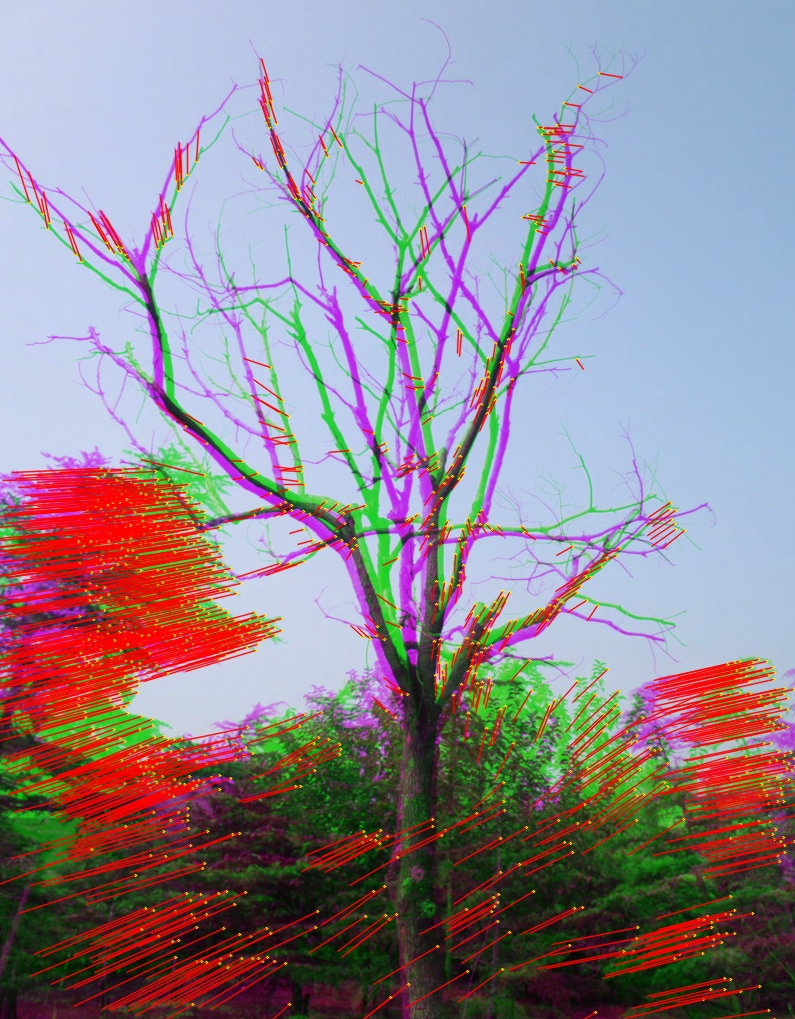
\includegraphics[height=10cm]{new.png}}
	\caption{Traditional PyrLK and Improved PyrLK}
	\label{fig:pyrlk}
\end{figure}


\clearpage
Algorithm \ref{alg:pyrlk} gives the pseudo-code of the improved PyrLK optical flow method:\\
\begin{algorithm}[H]
	\caption{Improved PyrLK}
	\label{alg:pyrlk}
	\begin{algorithmic}[1]
		\Require Image $I$,$J$,Point $\mathbf{u}$ in Image $I$
		\Ensure Corresponding point $\mathbf{v}$ in Image $J$
		\State Build the pyramidial representation of Image $I$ and $J$: $\{I^L\}_{L=0,...,L_m}$和$\{J^L\}_{L=0,...,L_m}$
		\State Initialize pyramid guess : $g^{L_{m}}=(g_x^{L_m}, g_y^{L_m})=(0,0)$
		\For{$L=L_m$to 0 with step of -1}
		\State Position point $\mathbf{u^L}$ in image $I^L$: $\mathbf{u}^L=(u_x,u_y)=\mathbf{u}/2^L$
		\State Assume $\mathbf{a_1}=(a_{11},a_{12},a_{13})\quad \mathbf{a_2}=(a_{21},a_{22},a_{23})\quad 
				\mathbf{b}=(d_x^L, d_y^L, 1$
		\State Define Similarity:
				\[ \epsilon(\mathbf{d^L})=\epsilon(d_x,d_y)=\sum_{x=u_x-\omega_x}^{u_x+\omega_x}\sum_{y=u_y-\omega_y}
				^{u_y+\omega_y}(I(x,y) - J(x+\mathbf{a_1}\cdot \mathbf{b},y+\mathbf{a_2}\cdot \mathbf{b}))^2.\]
				\State Least Squares to work out $d^L$,which let $\epsilon $ reach its minimum
		\State Guess on layer L-1: $g^{L-1}=2(g^L+d^L)$
		\EndFor
		\State Final optical flow vector: $\mathbf{d}=\mathbf{g^0}+\mathbf{d^0}$
		\State $\mathbf{v}=\mathbf{u+d}$
		\If{BackwardTrack$(\mathbf{v})$ = true}
			\If{MedianFilter$(\mathbf{v})$ = true}
				\State \Return $\mathbf{v}$
			\Else
				\State \Return NULL
			\EndIf
		\Else
			\State \Return NULL
		\EndIf
	\end{algorithmic}
\end{algorithm}

\section{本章小节}
\label{sec:conclusion}
本章首先介绍了光流法的由来,进而分析了LK光流法的思想和特点。然后对于基于图像金字塔的PyrLK光流法,它采用多分辨率图像层
来克服传统LK光流法无法捕捉图像中大块运动的缺陷。但是受缚于LK光流法的前提,该匹配算法只支持特征点的平移运动,由此带来很大
的束缚性。而且PyrLK光流法并没有对匹配的正确性进行验证,从而导致了很多错误的匹配对。基于这两方面的考虑,本章接着提出了支持
特征点旋转变换以及反向追踪的PyrLK光流法,这两个改进从根本上解决了PyrLK光流法的局限性,使PyrLK光流法的适用性和正确性都大大
的提升。本章的最后还给出了改进方法与传统方法的实验效果对比图。
